\documentclass{article}
\usepackage{listings}
\usepackage{listings}
\usepackage{color}
\usepackage{graphicx}
\usepackage{caption}
\graphicspath{ {./} }
\usepackage[top=1in, bottom=1.25in, left=1.25in, right=1.25in]{geometry}
\definecolor{mygreen}{rgb}{0,0.6,0}
\definecolor{mygray}{rgb}{0.5,0.5,0.5}
\definecolor{mymauve}{rgb}{0.58,0,0.82}
\lstset{ %
	backgroundcolor=\color{white},   % choose the background color; you must add \usepackage{color} or \usepackage{xcolor}; should come as last argument
	basicstyle=\footnotesize,        % the size of the fonts that are used for the code
	breakatwhitespace=false,         % sets if automatic breaks should only happen at whitespace
	breaklines=true,                 % sets automatic line breaking
	captionpos=b,                    % sets the caption-position to bottom
	commentstyle=\color{mygreen},    % comment style
	deletekeywords={...},            % if you want to delete keywords from the given language
	escapeinside={\%*}{*)},          % if you want to add LaTeX within your code
	extendedchars=true,              % lets you use non-ASCII characters; for 8-bits encodings only, does not work with UTF-8
	frame=single,	                   % adds a frame around the code
	keepspaces=true,                 % keeps spaces in text, useful for keeping indentation of code (possibly needs columns=flexible)
	keywordstyle=\color{blue},       % keyword style
	language=Octave,                 % the language of the code
	morekeywords={*,...},            % if you want to add more keywords to the set
	numbers=left,                    % where to put the line-numbers; possible values are (none, left, right)
	numbersep=5pt,                   % how far the line-numbers are from the code
	numberstyle=\tiny\color{mygray}, % the style that is used for the line-numbers
	rulecolor=\color{black},         % if not set, the frame-color may be changed on line-breaks within not-black text (e.g. comments (green here))
	showspaces=false,                % show spaces everywhere adding particular underscores; it overrides 'showstringspaces'
	showstringspaces=false,          % underline spaces within strings only
	showtabs=false,                  % show tabs within strings adding particular underscores
	stepnumber=2,                    % the step between two line-numbers. If it's 1, each line will be numbered
	stringstyle=\color{mymauve},     % string literal style
	tabsize=2,	                   % sets default tabsize to 2 spaces
	title=\lstname                   % show the filename of files included with \lstinputlisting; also try caption instead of title
}
\author{Polykarpos Thomadakis}
\title{Assignment 4 \\
	\large CS834 Introduction to Information Retrieval\\Fall 2017}
\begin{document}
	\maketitle
	\section*{Question 8.3}
	For one query in the CACM collection(provided at the book website), generate a ranking using Galago, and then calculate average precision, NDCG at 5 and 10, precision at 10, and the reciprocal rank by hand.
	\subsection*{Answer}
	For this assignment I used Galago in order to generate the rankings of the provided documents and then calculated the requested metrics based on the relevance file, also provided. The metrics were calculated based on the formulas that are presented on the book.
	The script that was written for the purposes of this assingnment is presented in listing \ref{lst:q83}. The user provides parameters such as: the files on which the search will be performed, the location of galago binary, the query id to generate metrics, the path to the galago index that will be created only once, a path to the xml query file and the path to the relevance file.
	A sample of the output of the program is shown on figure \ref{fig:q83} for the query number 8.
	\lstinputlisting[language=Python,caption={Script that generates the metrics of the assignment},label={lst:q83}]{galago_metrics.py}
	\begin{figure}[h]
		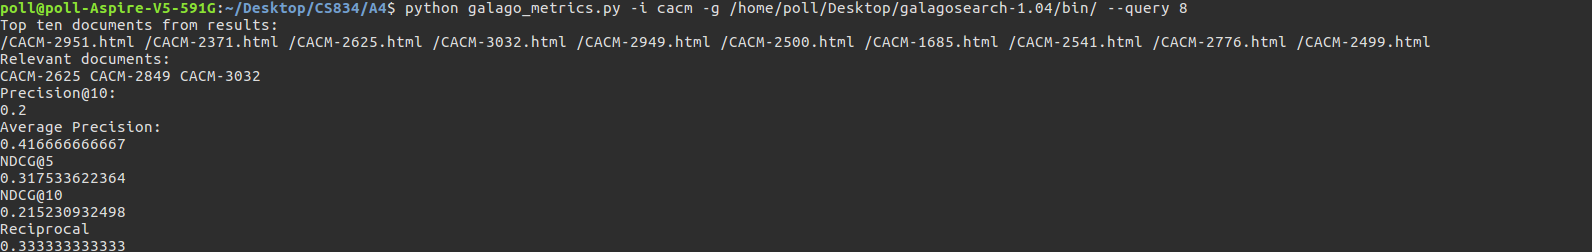
\includegraphics[width=\linewidth]{q83.png}
		\caption{Sample output of the script of this assignment}
		\label{fig:q83}
	\end{figure}
	\section*{Question 8.4}
	For two queries in the CACM collection, generate two uninterpolated recall precision graphs, a table of interpolated precision values at standard recall levels, and the average interpolated recall-precision graph.
	\section*{Answer}
	The chosen queries for this assignment are 3 and 5. The code can be seen in listing \ref{lst:q84}. The same command line arguments are given from the user, plus one more query index that is requested to extract metrics about. I used gnuplot for the graphs presented in figures \ref{fig:q84_un}, \ref{fig:q84_in} and \ref{fig:q84_avg_in}. The table with the interpolated precision values on standard recall values is shown in table \ref{tb:int_values}.
	\lstinputlisting[language=Python,caption={Script that generates the graphs of the assignment},label={lst:q84}]{recall_graphs_gen.py}
	\begin{figure}[h]
		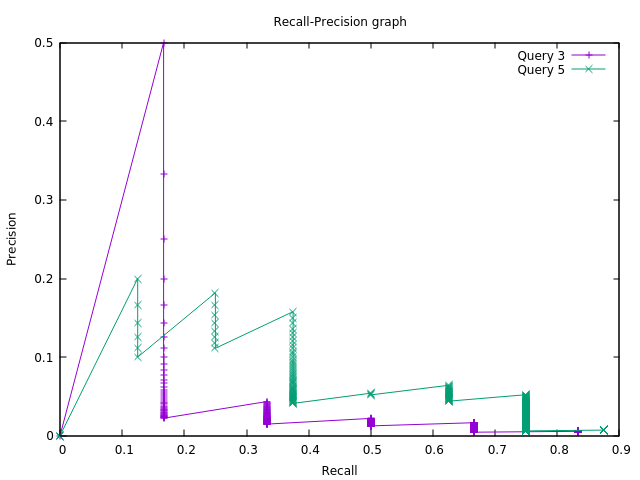
\includegraphics[width=.85\linewidth]{unint_q84.png}
		\caption{The uninterpolated recall-precision graphs for the two queries}
		\label{fig:q84_un}
	\end{figure} 
	\begin{figure}
		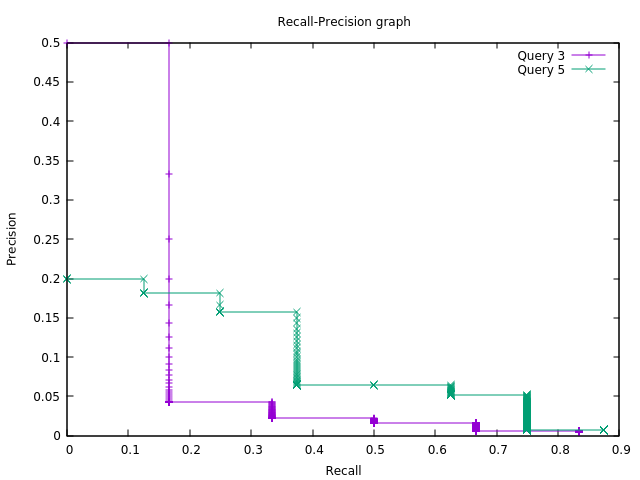
\includegraphics[width=.85\linewidth]{int_q84.png}
		\caption{The interpolated recall-precision graphs for the two queries}
		\label{fig:q84_in}
	\end{figure}
	\begin{figure}
		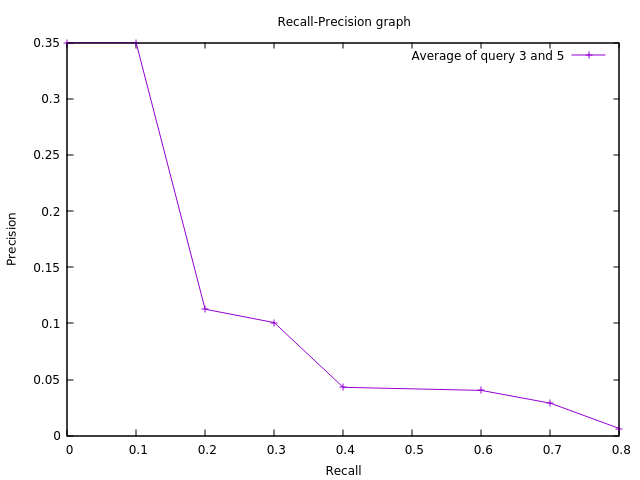
\includegraphics[width=.85\linewidth]{avg_int_q84.png}
		\caption{The interpolated average recall-precision graph for the two queries}
		\label{fig:q84_avg_in}
	\end{figure}
	\begin{table}[h]
		\centering
		\caption{Table with the interpolated values in standard recall values}
		\label{tb:int_values}
		\begin{tabular}{|c|c|c|}
			\hline
			0.1 & 0.5              & 0.2              \\ \hline
			0.2 & 0.0434782608696  & 0.181818181818   \\ \hline
			0.3 & 0.0434782608696  & 0.157894736842   \\ \hline
			0.4 & 0.0220588235294  & 0.0641025641026  \\ \hline
			0.6 & 0.0165289256198  & 0.0641025641026  \\ \hline
			0.7 & 0.00563063063063 & 0.0521739130435  \\ \hline
			0.8 & 0.00563063063063 & 0.00713557594292 \\ \hline
		\end{tabular}
	\end{table}
	\section*{Question 8.5}
	Generate the mean average precision, recall-precision graph, average NDCG at 5 and 10, and precision at 10 for the entire CACM query set.
	\subsection*{Answer}
	Again, I used the formulas provided on the book to generate the metrics requested for the whole cacm query set. The script I wrote for this purpose is presented in listing \ref{lst:q85}. The values generated for this assignment can be seen in figure \ref{fig:q85_1} and the average interpolated recall-precision graph for the entire query set in figure \ref{fig:q85_2}.
	\lstinputlisting[language=Python,caption={Script to generate the metrics of the assignment},label={lst:q85}]{cacm_metrics.py}
	\begin{figure}[h]
		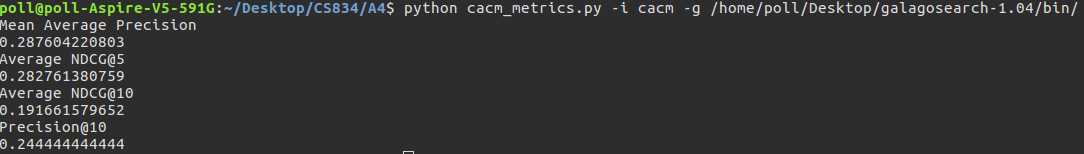
\includegraphics[width=\linewidth]{q85.png}
		\caption{Metrics requested for the entire cacm query set}
		\label{fig:q85_1}
	\end{figure}
	\begin{figure}[h]
		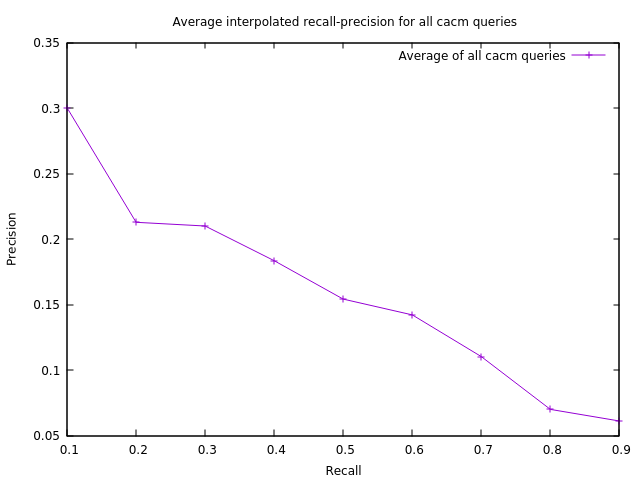
\includegraphics[width=\linewidth]{q85_1.png}
		\caption{The average interpolated recall-precision graph for the entire query set}
		\label{fig:q85_2}
	\end{figure}
	
	\section*{Question 8.7}
	Another measure that has been used in a number of evaluations is R-precision. This is defined as the precision at R documents, where R is the number of relevant documents for a query. It is used in situations where there is a large variation in the number of relevant documents per query. Calculate the average R-precision for the CACM query set and compare it to the other measures.
	\subsection*{Answer}
	The script to calculate the R-precision and compare it with other metrics can be seen in listing \ref{lst:q87}. Figure \ref{fig:q87} shows the R-precision value as well as the other metrics of the CACM query set.
	\lstinputlisting[language=Python,caption={Script to generate the R-precision metric and compare it with others},label={lst:q87}]{r_precision.py}
	\begin{figure}[h]
		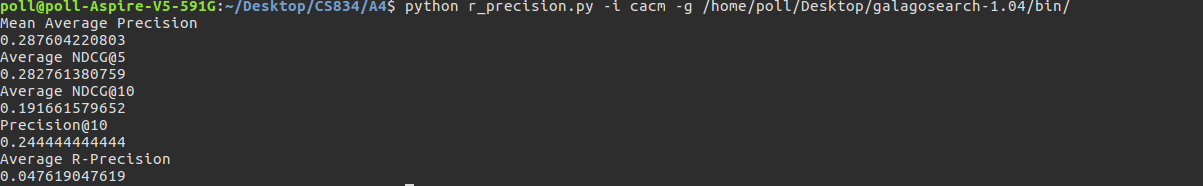
\includegraphics[width=\linewidth]{q87.png}
		\caption{The comparison between R-precision, MAP, NDCG@5, NDCG@10 and Precision@10}
		\label{fig:q87}
	\end{figure}
	\section*{Question 8.9}
	For one query in the CACM collection, generate a ranking and calculate
	BPREF. Show that the two formulations of BPREF give the same value.
	\subsection*{Answer}
	I use the two formulas of the book to calculate BPREF for the query 2. They both give the same results as the book states and can be seen in figure \ref{fig:q89}. BPREF1 refers to the formula: 	         $$BPREF1=\frac{1}{R}\sum_{dr}^{}(1-\frac{N_{dr}}{R})$$ 
	and BPREF2 to the formula:
	$$BPREF2=\frac{P}{P+Q}$$ 
	The code for this assignment is shown in listing \ref{lst:q89}.
	\begin{figure}[h]
		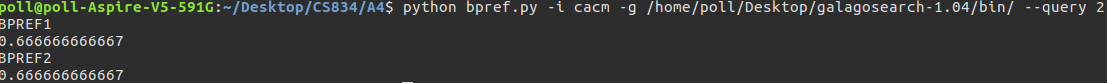
\includegraphics[width=\linewidth]{q89.png}
		\caption{BPREF as generate by the two formulas in the book}
		\label{fig:q89}
	\end{figure}
	\lstinputlisting[language=Python,caption={Script to generate the BPREF metric with both formulas},label={lst:q89}]{bpref.py}
	
\end{document}